\chapter{实验材料与研究方法}

\section{实验材料属性}
本实验用的是真空自耗两次熔炼所得的钛合金板,其化学成分参数与室温(20℃)力学性能参数如\ref{sec:mytc4chem}与\ref{sec:mytc4machin}所示:
\begin{table}[htbp]
	\centering
	\caption{试样的化学成分参数}
	\label{sec:mytc4chem}
	\begin{tabular}{cccccccc}
		\toprule
		元素($ \% $) & Al & V &Fe &C& O& N &H \\ \midrule
		实际含量 & 6.12&4.06 &0.13 &0.012&0.112&0.009&0.004  \\
		标准要求 &$ 5.5\sim 6.75 $ & $ 3.5\sim 4.5 $&$ \le 0.30 $ & $ \le 0.05 $&$ \le 0.20 $&$ \le 0.03$ &$ \le 0.015 $ \\ \bottomrule
	\end{tabular}
\end{table}
\begin{table}[htbp]
	\centering
	\caption{试样的力学性能参数}
	\label{sec:mytc4machin}
	\begin{tabular}{cccc}
		\toprule
		力学性能& 抗拉强度$Mpa  $& 屈服强度$ Mpa $&断后伸长率$ \% $\\ \midrule
		实测值 & 983 &902 & 13\\
		标准值 &$ \ge 895 $&$ \ge 830 $&$ \ge 10 $ \\ \bottomrule
	\end{tabular}
\end{table}

%
%\begin{figure}[!htbp]
%	\centering
%	\begin{minipage}[t]{0.68\textwidth}
	%		\centering
	%		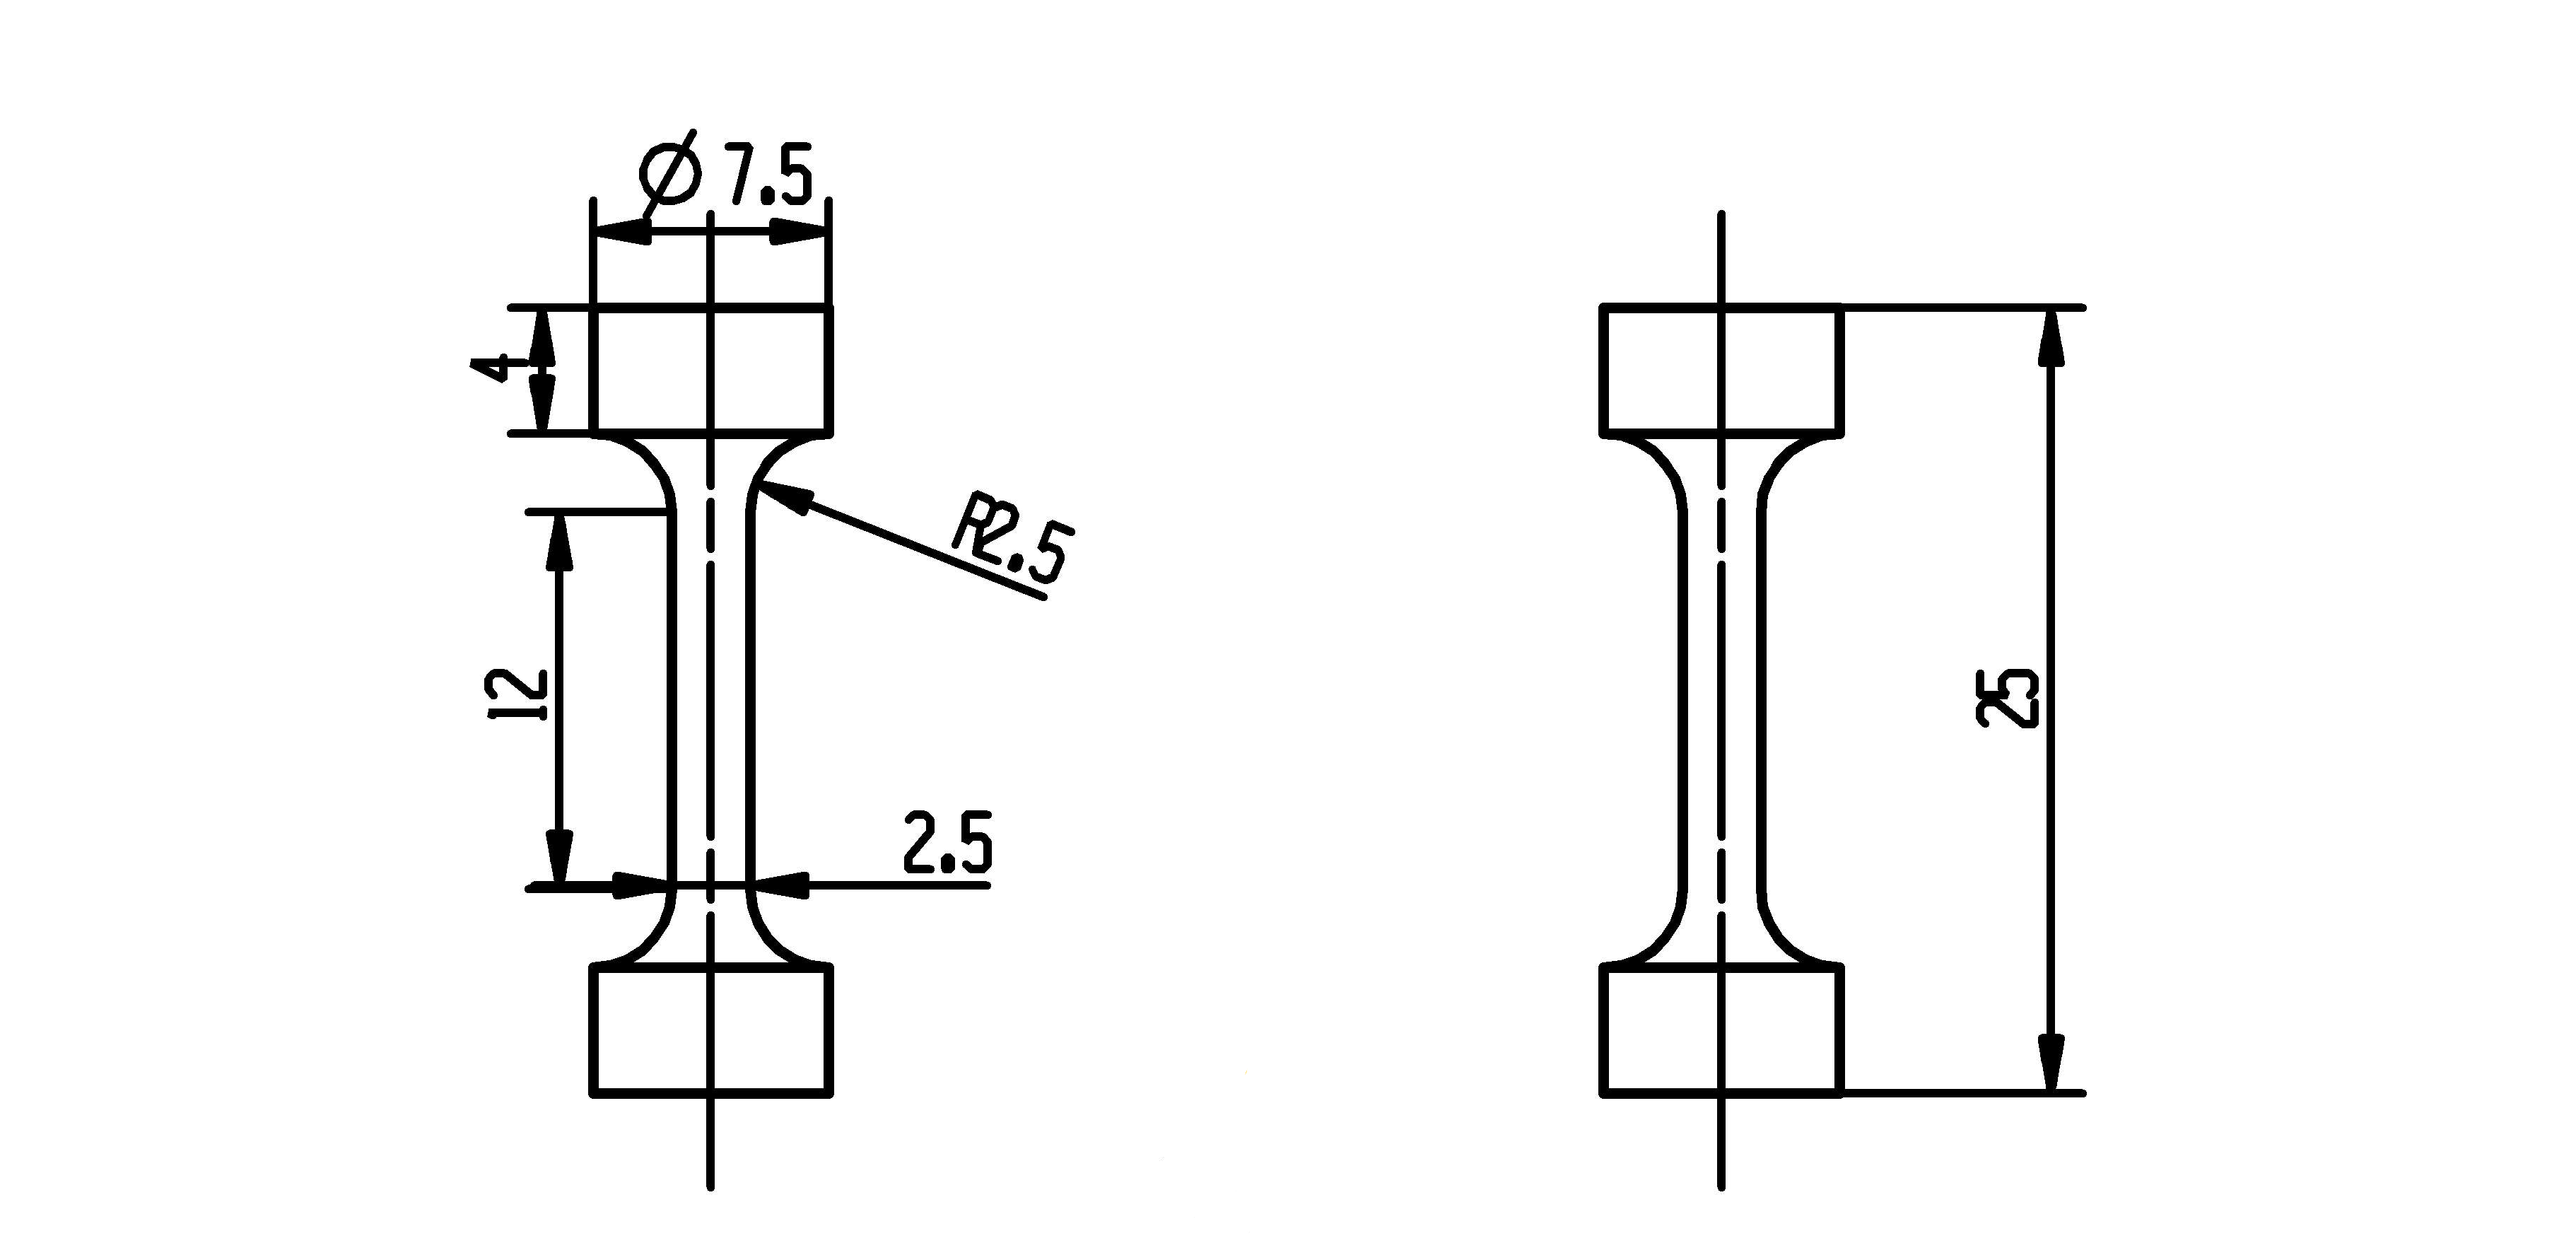
\includegraphics[width=6cm]{pic/试样}
	%		\caption{试样的尺寸参数}
	%		\label{fig:试样尺寸}
	%	\end{minipage}
%	\begin{minipage}[t]{0.3\textwidth}
	%		\centering
	%		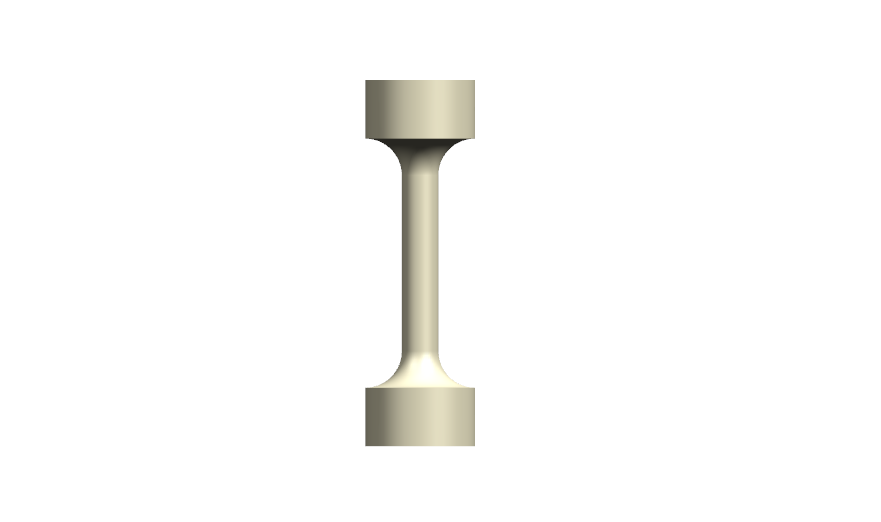
\includegraphics[width=6cm]{pic/模型}
	%		\caption{试样的三维模型}
	%		\label{fig:试样的三维模型}
	%	\end{minipage}
%%	\caption{试样参数}
%\end{figure}

\subsection{$\beta$转变温度的计算}
$\beta$转变温度是钛合金的重要参数之一,它是制定钛合金的热机械工艺和热处理工艺的重要依据,相变过程如\ref{sec:Tc4betachange}所示。

\begin{table}[htbp]
	\centering
	\caption{\ti 合金$ \alpha+\beta \to \beta $转变时发生的相变及存在的相}
	\label{sec:Tc4betachange}
	\begin{tabular}{ccc}
		\toprule 室温相 & 相变过程 & 高温相 \\
		\midrule$\alpha-\mathrm{Ti}$ & $\alpha-T i \rightarrow \beta-T i$ & $\beta-\mathrm{Ti}$ \\
		$\alpha-\mathrm{Ti}-\mathrm{Al}$ & $\alpha-\mathrm{Ti}-\mathrm{Al} \rightarrow \beta-\mathrm{Ti}+\beta-\mathrm{Ti}-\mathrm{Al}$ & $\beta-\mathrm{Ti}, \beta-\mathrm{Ti}-\mathrm{Al}$ \\
		$\beta- \mathrm{Ti}-\mathrm{V}$ & $\beta-\mathrm{Ti}-\mathrm{V} \rightarrow \beta^{-} \mathrm{Ti}-\mathrm{V}$ & $\beta-\mathrm{Ti}-\mathrm{V}$ \\
		\bottomrule
	\end{tabular}
\end{table}

$\beta$转变温度于TC4合金组织转变的关系非常密切,对于TC4合金热处理工艺的设计至关重要。郭凯\cite{guokaiTC4taihejinrechuligongyideyanjiuxianzhuangjijinzhan2021}等人表示:当固溶温度高于 $\beta$ 相变时的温度时,合金的强度伴随温度的增加而下降,而且残余应力也开始大幅度的降低;当固溶温度在相变点以下时,合金的强度伴随温度的增加而增加。但是徐戊矫、谭玉全\cite{xujianGurongshixiaogongyiduiTC4taihejinzuzhijixingnengdeyingxiang2014}却表明:在相变点以下,随着退火温度的升高,材料的 强度、塑性和冲击韧性呈降低趋势。之所以会出现这种完全相反的结论,很可能是研究者对于相变点的具体值定义不清晰导致的,可见相变点的确定在固溶处理过程中是非常关键的。


关于$\beta$转变温度的具体值,目前广泛认同的是位于975℃附近,但是由于不同试样的合金元素的种类与含量的差异,尤其是局部化学成分的差异,使得不同研究人员实际测得的相变点温度有所差异\cite{wangtaoTC4hejinxiangbianwendujiancezhongjieguobuyizhiyuanyinfenxi2013}。姚德人等\cite{yaoderenTc4taihejinxiangbiandiandeceding1975}表明相变温度为975℃到980℃之间,此时的合金拥有最低的硬度,当温度略大时会发生$\beta$晶粒的显著长大;相变点以下50℃以内水淬,可以得到不同数量的初生$ \alpha $和马氏体$ \alpha^{\prime} $,而后再进行低温退火时,马氏体$ \alpha^{\prime} $又会转变为稳定的次生$ \alpha$和$ \beta $,可以得到较好的综合性能%\footnote{\color{black}此文章写于1975年,但是仍然非常有参考价值}。
刘伟东等人\cite{liuweidongTC4hejinVzhuanbianwendudejinxiangfacedingyulilunjisuan2014}通过连续升温金相法,使用EET\footnote{Empirical Electron Theory of solids and molecules“固体与分子经验电子理论”(简称余氏理论)}模型建模测得了\ti 合金的相变温度为974.58℃;孙宇、曾卫东等人\cite{sunyuYingyongrengongshenjingwangluoyanjiuhuaxueyuansuduitaihejinxiangbiandiandeyingxiang2010}通过人工神经网络ANN技术,运用反向传播算法,建立了三层神经网路-钛合金相变预测模型,最终预测得到在绝对误差为9.8℃的情况下,TC4的相变点为994.8℃。

现阶段确定$ \beta $相变点的常见计算方法\cite{zhuhongTaihejinaVxiangbiandiandejizhongceshifangfatantao2013}主要有:连续升温金相法、X 射线衍射法、电阻法、等热膨胀法、元素含量法和神经网络模型预测预测法\cite{renchiqiangGurongshixiaoduiTC4taihejinxianweizuzhihelixuexingnengdeyingxiang2022}等。元素含量法是据合金中各元素对相变温度的影响\cite{ananyaLocationBasedIntelligent2011}利用经验公式\ref{jingyan}来对相变点进行推算;膨胀法是根据金属在加热过程中用发生相变时新相与母相的膨胀系数不同或比容 发生变化而确定相变点;金相法主要用于相变温度的检验,主要步骤是:先在计算得到的(比如元素含量法)理论相变温度附近每隔5°C或10°C热处理1个样品,然后在金相显微镜下观察到无剩余$\alpha$相的试样,将比该试样热处理温度低5°C的温度计为钛合金的$\alpha+\beta/\beta$相转变温度。各种方法各有优缺点,实验者应根据实际条件进行选取。
\begin{equation}
	T_\beta=885^{\circ} \mathrm{C}+\sum \textit{ 各元素含量 } \times \textit{ 各元素含量对 }(\alpha+\beta) / \beta \textit{ 相变点的影响 }
	\label{jingyan}
\end{equation}
其中885℃为纯钛的相变点。

在上述的各种测试方法中,元素含量法作为一种最为常用的方法,由于其简单且准确的特点,得到了较高频率的使用,大多数TC4合金热处理相关试验都使用了元素含量法进行相变点的计算\cite{LiuLeiTi6Al4VTaiHeJinBuTongReChuLiFangFaDeShiYanYuFuHeCaiLiaoLiXueXingNengFenXi2022,zouhaibeiTC4taihejinrechuliqianghuagongyijixiangbianhangweiyanjiu2019,liutaoRechuliduiTC4taihejindongtailixuexingnengheweiguanzuzhideyingxiang,baoxuechunRechuligongyiduiTC4taihejinzuzhihelixuexingnengdeyingxiang2019,wangpuqiangButongrechuligongyixiajiguangzengcaizhizaoTC4taihejinzuzhiyuxingnengyanjiujinzhan2020},得到的结果都十分准确,具有较高的可信度。故本设计采用此方法来对实验材料的$\beta$转变温度进行推算,元素含量如上\ref{sec:mytc4chem}所示。通过计算不同元素对于相变点温度的影响,得到\ref{sec:chem4ti}:

\begin{table}[htbp]
	\centering
	\caption{部分元素含量对钛合金相变点的影响}
	\label{sec:chem4ti}
	\begin{tabular}{cccc}
		\hline 元素名称 & 元素含量 $(\mathrm{Wt} \%)$ & 差值&累积值 \\
		\hline $\mathrm{Al}$ & $2.0 \sim 7.0$ & 29+$23.0^{\circ} \mathrm{C} / 1.0 \%$ & $+123.76^{\circ} \mathrm{C}$ \\
		$\mathrm{V}$ & $0 \sim 10.0$ & $-14.0^{\circ} \mathrm{C} / 1.0 \%$ & $-56.84^{\circ} \mathrm{C}$ \\
		$\mathrm{Fe}$ & $0 \sim 15.0$ & $-16.5^{\circ} \mathrm{C} / 1.0 \%$ & $-2.145^{\circ} \mathrm{C}$
		\\
		$\mathrm{C}$ & $0 \sim 0.15$ & $+2.0^{\circ} \mathrm{C} / 0.01 \%$ &$ +2.4^{\circ} \mathrm{C} $\\
		$\mathrm{O}$ & $0 \sim 1.0$ & $+2.0^{\circ} \mathrm{C} / 0.01 \%$& $ +22.4^{\circ} \mathrm{C} $\\
		$\mathrm{~N}$ & $0 \sim 0.5$ & $+5.5^{\circ} \mathrm{C} / 0.01 \%$& $ +4.95^{\circ} \mathrm{C} $\\
		$\mathrm{H}$ & $0 \sim 0.50$ & $-5.5^{\circ} \mathrm{C} / 0.01 \%$ &$ -2.2^{\circ} \mathrm{C} $\\
		\hline
	\end{tabular}
\end{table}

\begin{equation}
	\begin{aligned}
		T_\beta&=885^{\circ} \mathrm{C}+\sum (\delta_{Al}+\delta_{V}+\delta_{Fe}+\delta_{C}+\delta_{O}+\delta_{N}+\delta_{H})\\
		&= 885^{\circ} \mathrm{C}+(123.76-56.84-2.145+2.4+22.4+4.95-2.2)^{\circ} \mathrm{C}\\
		&=885^{\circ} \mathrm{C}+92.325^{\circ} \mathrm{C}\\
		&=977.325^{\circ} \mathrm{C}
	\end{aligned}
\end{equation}

最终通过计算法得到的相变点温度为$977.325^{\circ} \mathrm{C} $,与广泛认同的相变点温度值相差$\delta=\frac{977.325-975}{975}=0.238\% $,可见还是比较符合现实情况的,故本实验选择此温度作为热处理实验的基准温度。


\subsection{试样设计与加工}
本设计选择了尺寸较小的试样来进行实验:整体尺寸为$ 25mm\times 7.5mm $,厚度为1.3mm,呈现为两端略大,中间平行的骨头状。该类型的小件试样不仅可以节约材料,特殊的形状也便于进行后续的力学拉伸试验,满足实验要求,十分适合于昂贵金属的性能试验。参数如\ref{fig:试样尺寸}所示:
%3-28日上午,经过老师说明,由于试样为板材,加工成圆柱较为困难,故加工成二位平面的“狗骨头”

\begin{figure}[h!]
	\centering
	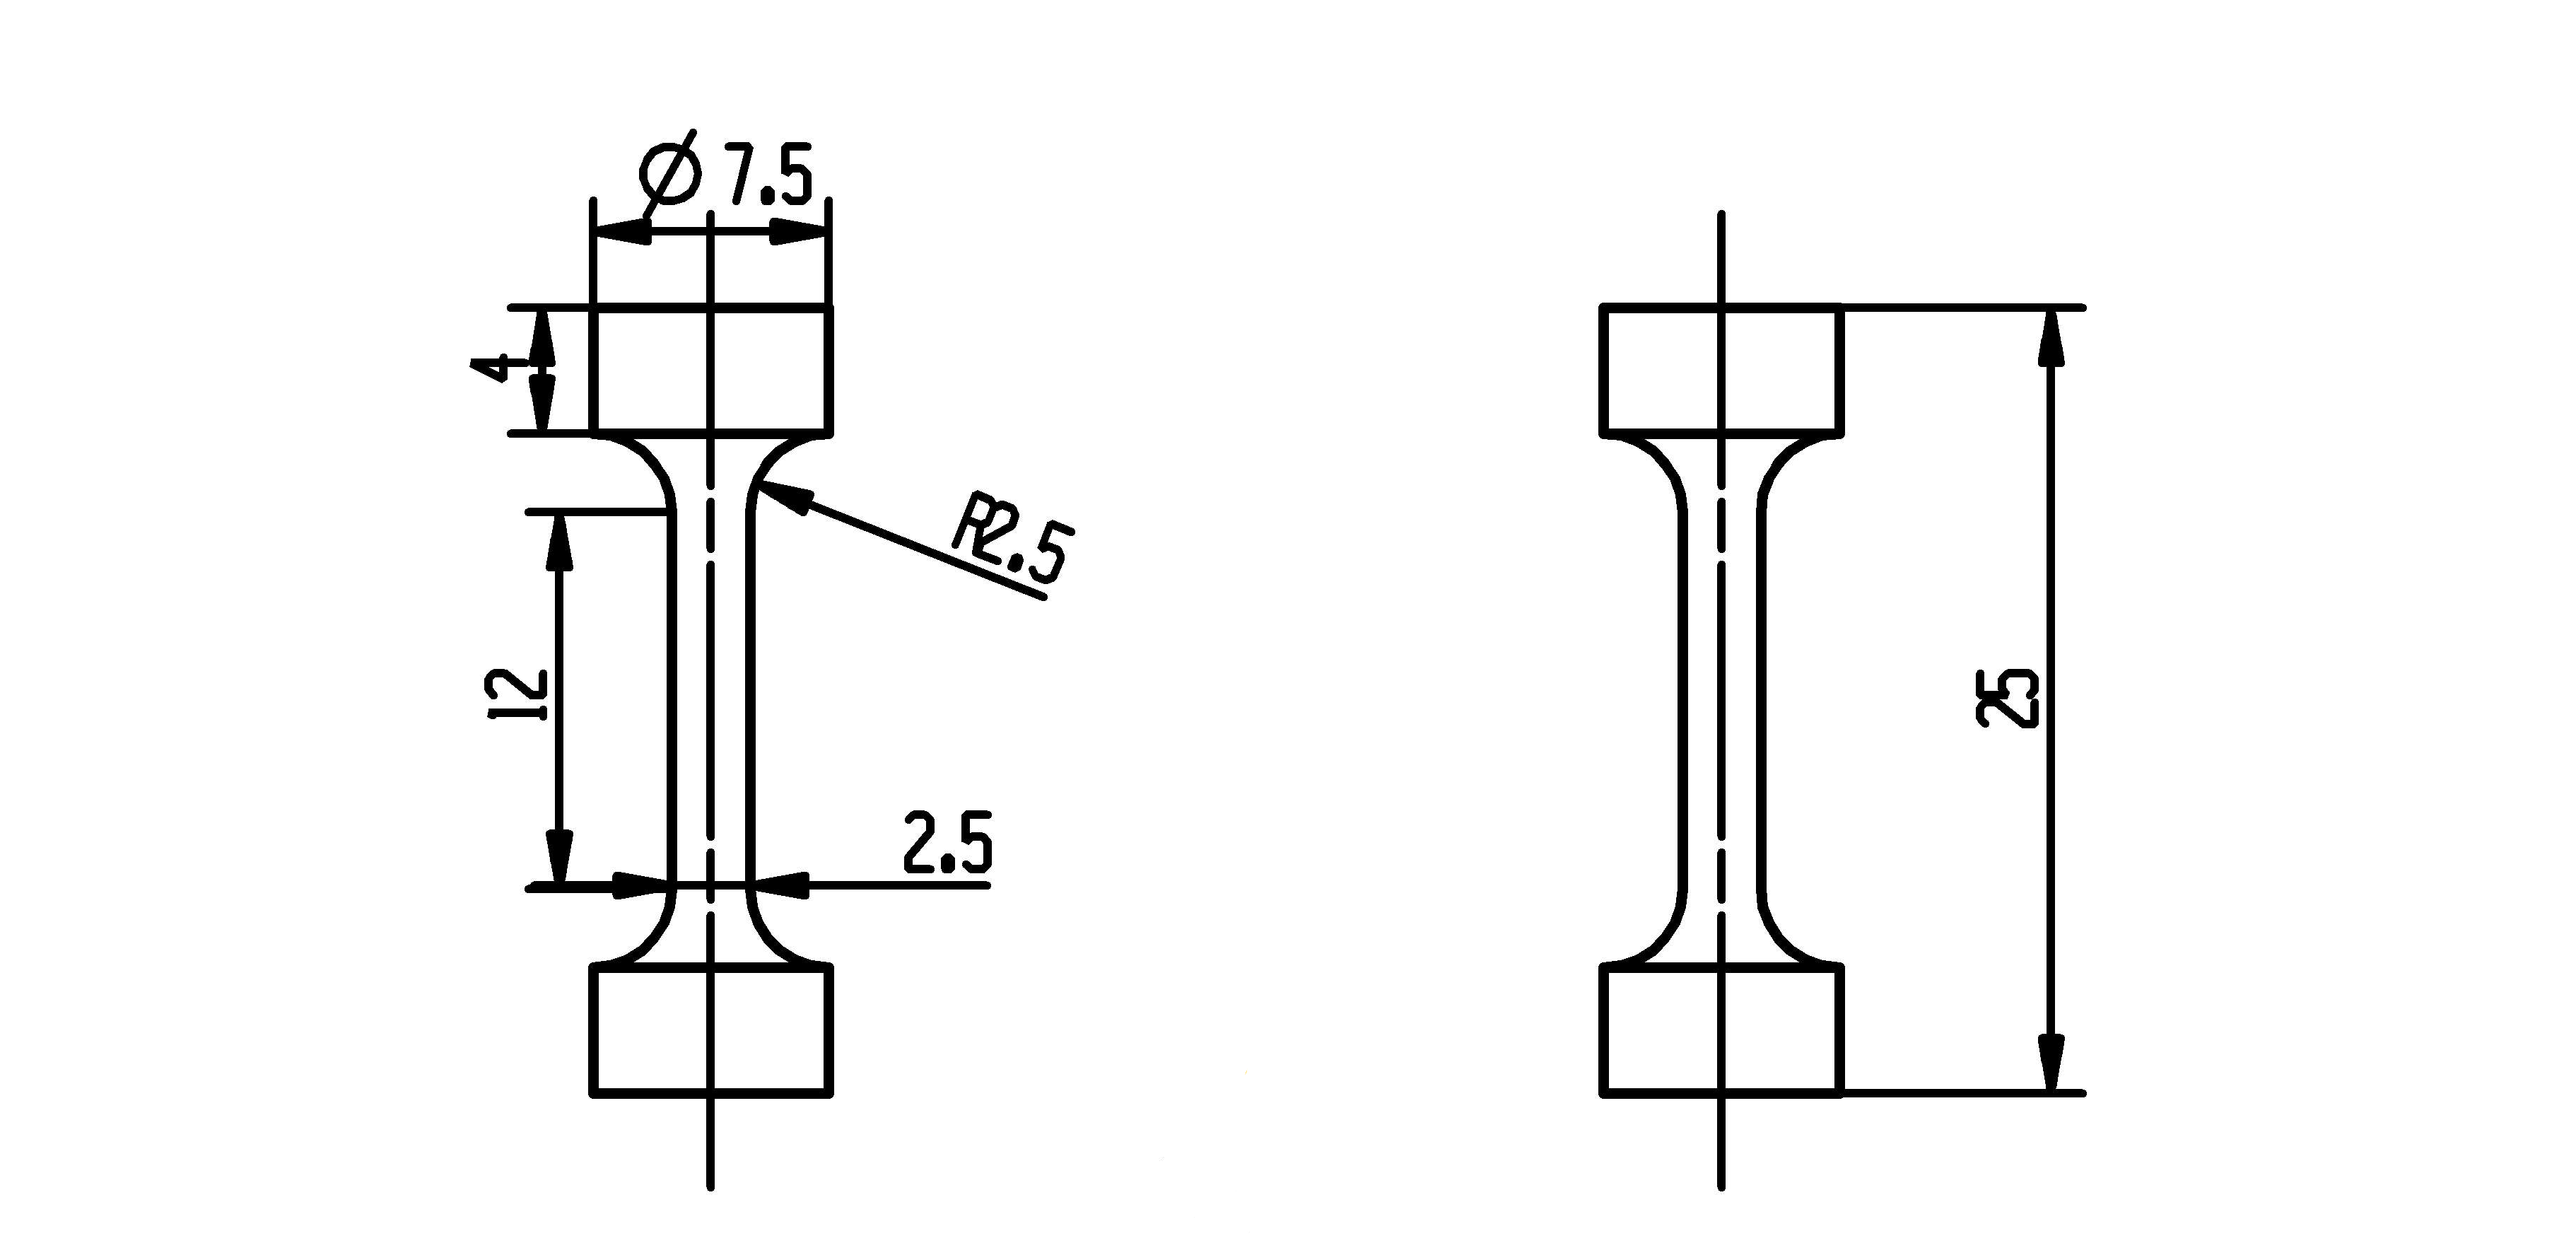
\includegraphics[width=0.7\linewidth]{pic/试样}
	\caption{试样的尺寸参数}
	\label{fig:试样尺寸}
\end{figure}

原始的材料板材$ 250mm\times 150mm $的板材,为了加工出来目标形状的试样,本设计选用电火花线切割(Wire cut Electrical Discharge Machining)的方法进行加工。

在加工的准备阶段,为了达到节约材料、提高材料的利用率的目标,设计了如\ref{fig:badway}所示的刀路,让式样尽可能密集排列,用最少的刀路切割来最多的试样。但在实际加工阶段,发现\ref{fig:badway}的刀路设计没有考虑夹具的安装位置、$ 0.05mm $粗的线切割用钼丝的尺寸,不要具备加工可行性。
\begin{figure}[h!]
	\centering
	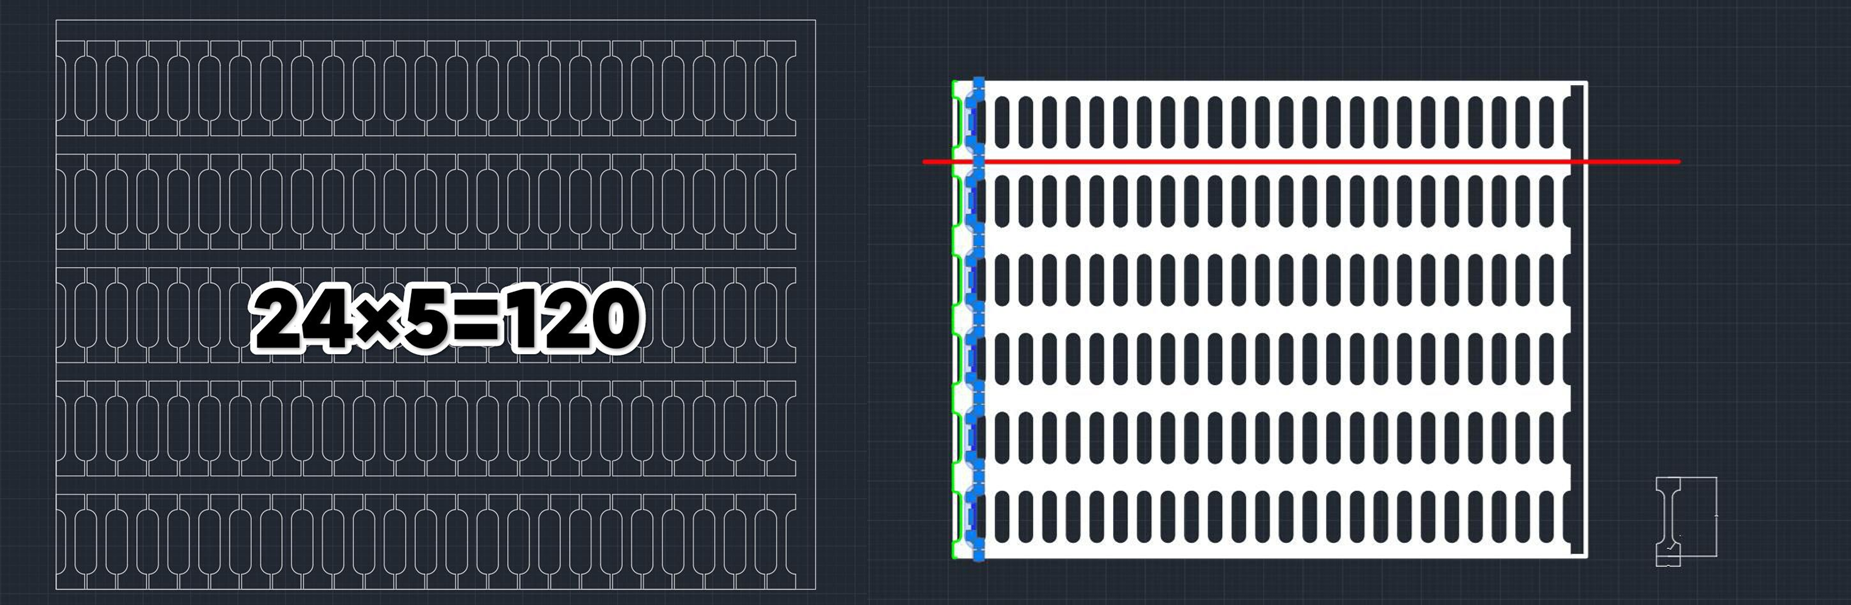
\includegraphics[width=0.8\linewidth]{pic/刀路初步}
	\caption{初步设计的刀路}
	\label{fig:badway}
\end{figure}

加工前的最后阶段,在综合考虑了加工方法、设备特点、加工成本%\footnote{上述设计的小式样,每个加工费25元}
等因素后,本实验加工方式改进为:整体板材板切割成八小板;小板堆叠装夹在一起进行加工,如图\ref{fig:goodway}所示,最终切割得到了$ 7\times 8=56 $个试样。
\begin{figure}[h!]
	\centering
	\subfigure[堆叠式切割设计]{
		\label{fig:goodway}
		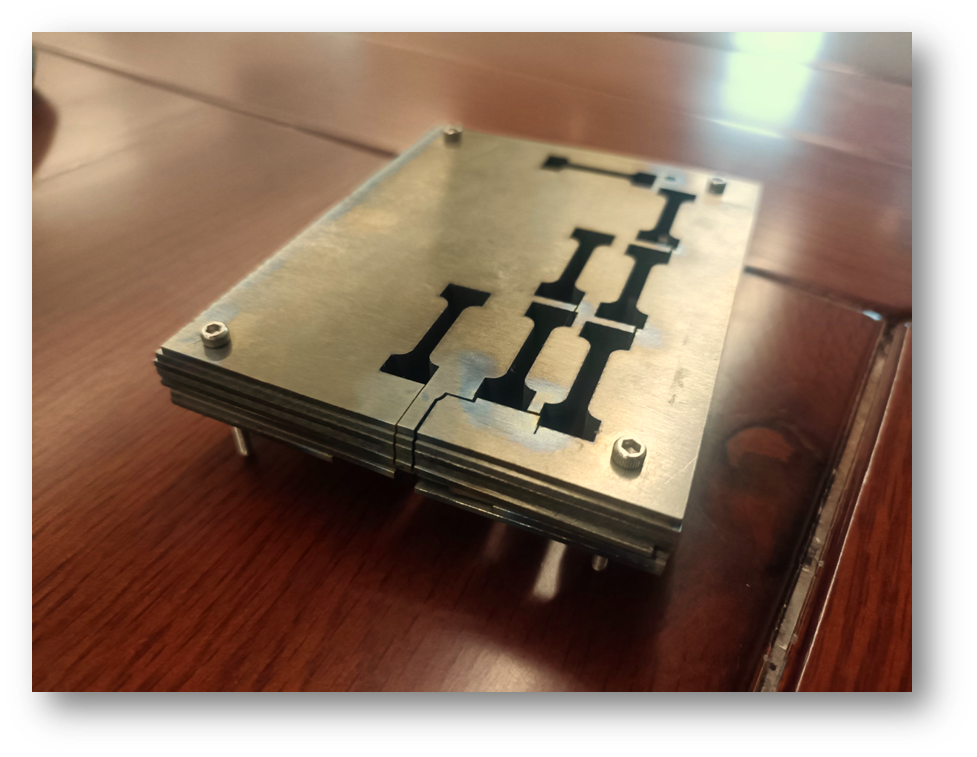
\includegraphics[width=0.4\linewidth]{pic/堆叠式切割}}
	\hspace{0.2in} % 两图片之间的距离
	\subfigure[切割后的部分试样]{
		\centering
		\label{fig:mytc4bone}
		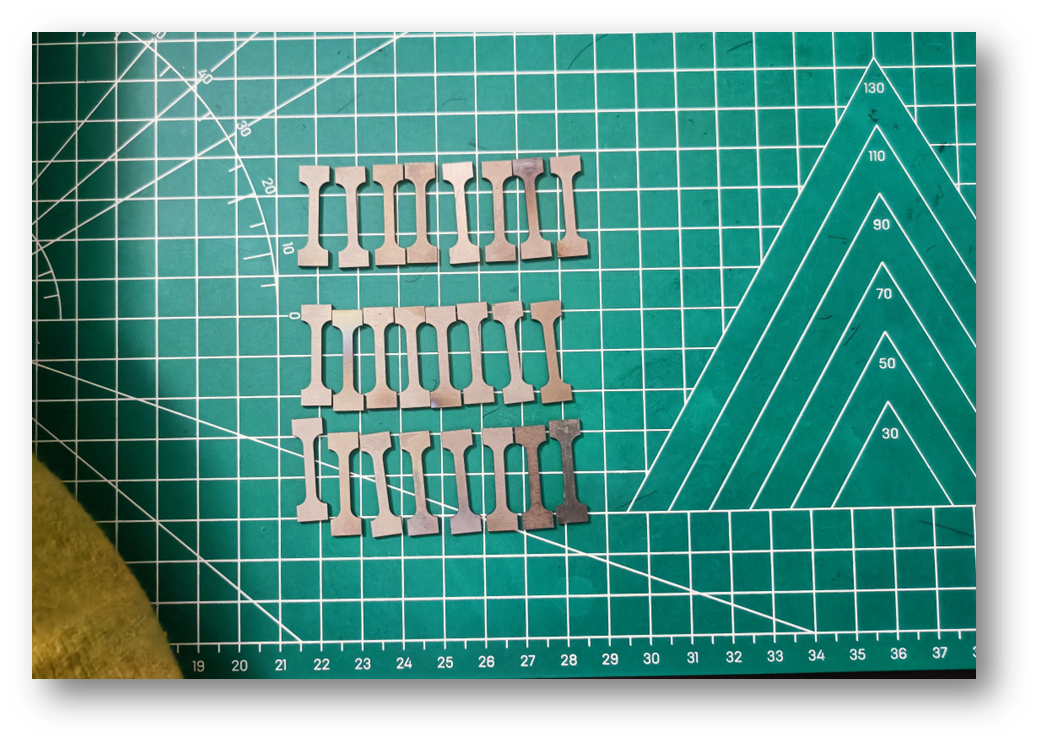
\includegraphics[width=0.45\linewidth]{pic/切割后的试样}}
	\caption{切割方法与切割结果}
\end{figure}

\section{整体实验路线}
本设计采用实验+分析的研究方法,热处理在\text{\color{teal}JC-MF12-30}%\footnote{该箱式电阻炉(也称为马弗炉)制造商为$\text{青岛聚创}^\text{\textregistered}  $环保集团有限公司,设备编号为803229}
型箱式电阻炉中进行。热处理完成后,进行了断裂形态的显微组织分析、拉伸力学试验、仪器冲击试验、X射线衍射(XRD)试验和环境扫描电子显微镜(ESEM)观察,研究的路线如\ref{fig:roadmap}所示:

\begin{figure}[h!]
	\centering
	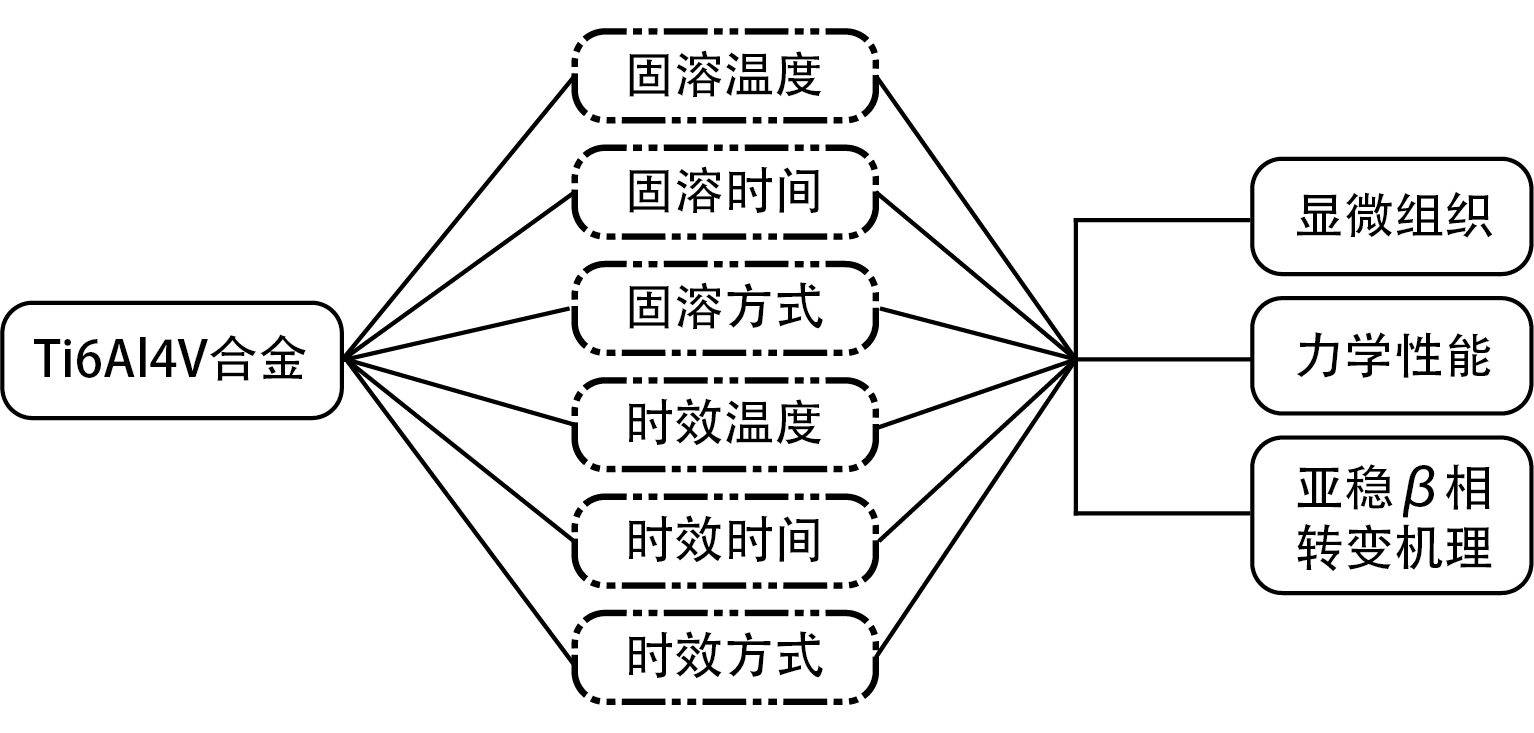
\includegraphics[width=0.8\linewidth]{pic/路线图}
	\caption{研究路线图}
	\label{fig:roadmap}
\end{figure}
\section{钛合金固溶时效热处理试验}
本实验分先后两次进行热处理:先进行固溶处理,随后进行时效处理,方案路线如\ref{fig: heatway}所示。
\begin{figure}[h!]
	\centering
	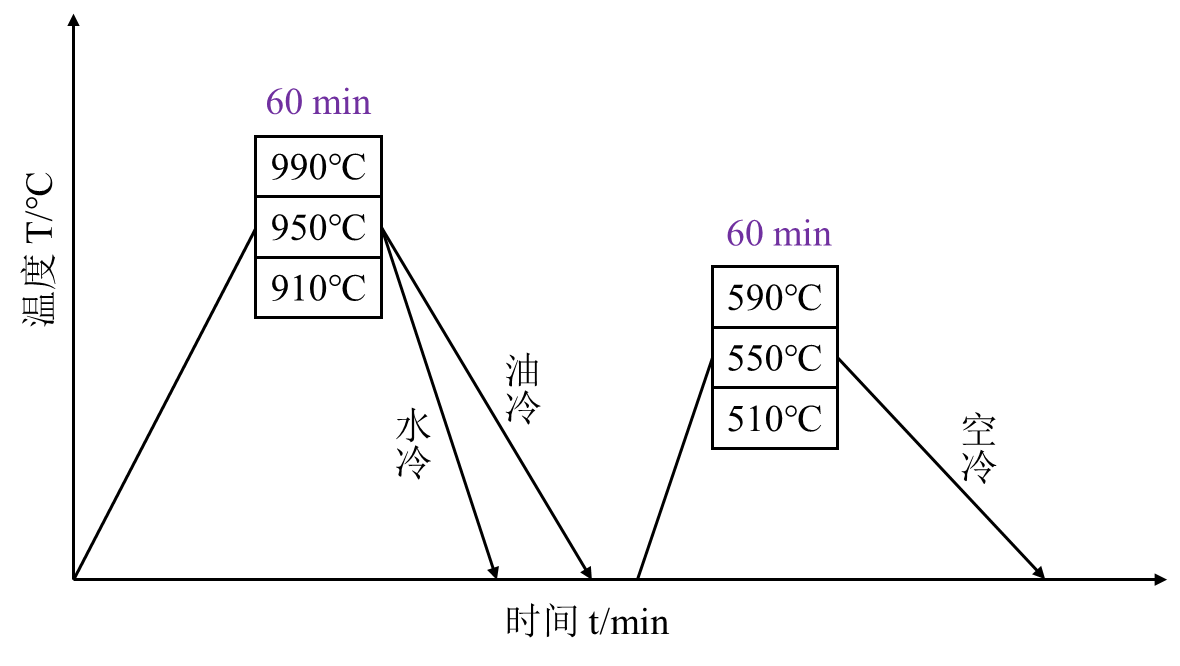
\includegraphics[width=0.7\linewidth]{pic/处理路线}
	\caption{固溶-时效热处理试验路线}
	\label{fig: heatway}
\end{figure}

热处理实验所用的设备为\text{\color{teal}JC-MF12-30}型箱式电阻炉,外观如\ref{fig: mymuffle}所示,设备规格如\ref{sec:mymuffle}所示:


\begin{table}[htbp]
	\centering
	\caption{\text{\color{teal}JC-MF12-30}型箱式电阻炉的规格}
	\label{sec:mymuffle}
	\begin{tabular}{cc}
		\toprule
		参数&值\\
		\midrule
		型号&JC-MF12-30\\
		编号&803229\\
		电压&380V\\
		功率&12KW\\
		常用温度&1150℃\\
		最高温度&1200℃\\
		炉膛尺寸& 500$ \times $ 300$ \times $ 200(mm) \\
		制造日期&2023年2月\\
		制造商& $\text{青岛聚创}^\text{\textregistered}  $环保集团有限公司\\
		\bottomrule
	\end{tabular}
\end{table}
固溶实验需要淬火,用到的淬火液体如\ref{fig:淬火用液体}所示:
\begin{figure}[h!]
	\centering
	\subfigure[马弗炉外形]{
	\label{fig: mymuffle}
	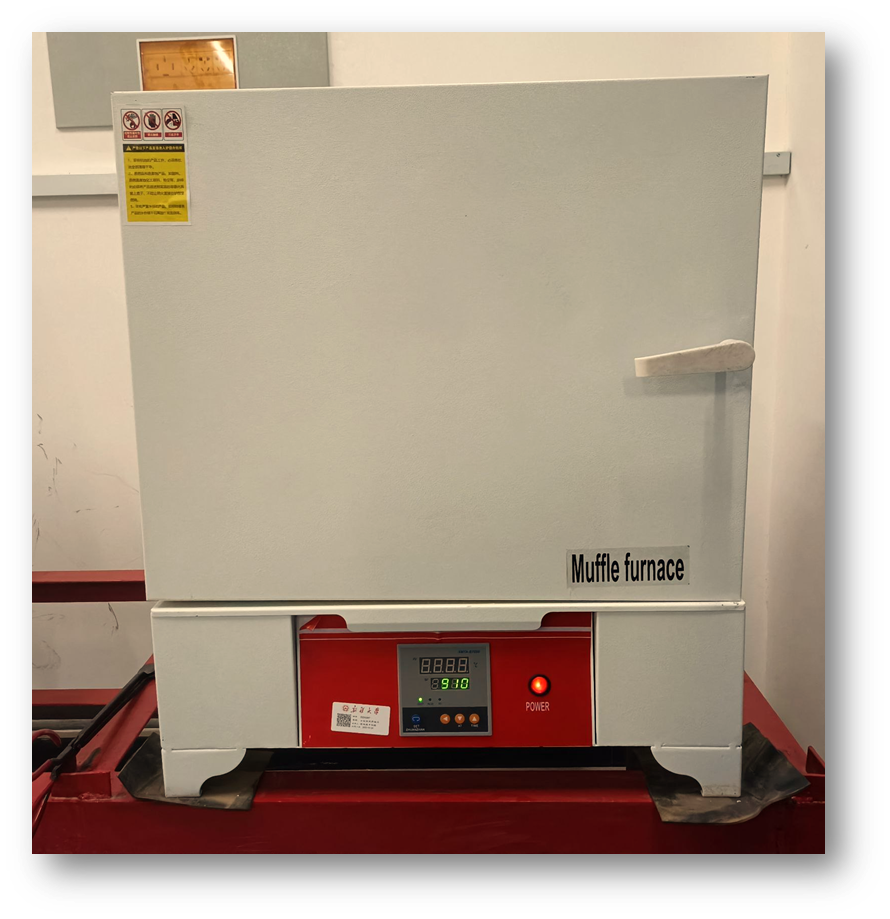
\includegraphics[scale=0.2]{pic/马弗炉}}
\hspace{0.01in} % 两图片之间的距离
	\subfigure[水淬液]{
		\label{fig:subfig:WCfluid}
		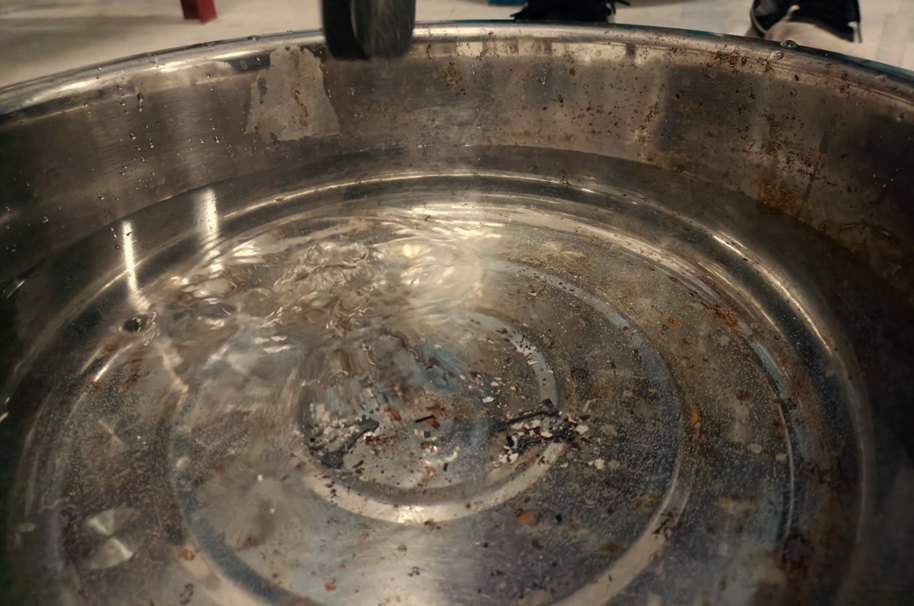
\includegraphics[scale=0.25]{pic/水淬液}}
	\hspace{0.01in} % 两图片之间的距离
	\subfigure[淬火油]{
		\label{fig:subfig:OCfluid}
		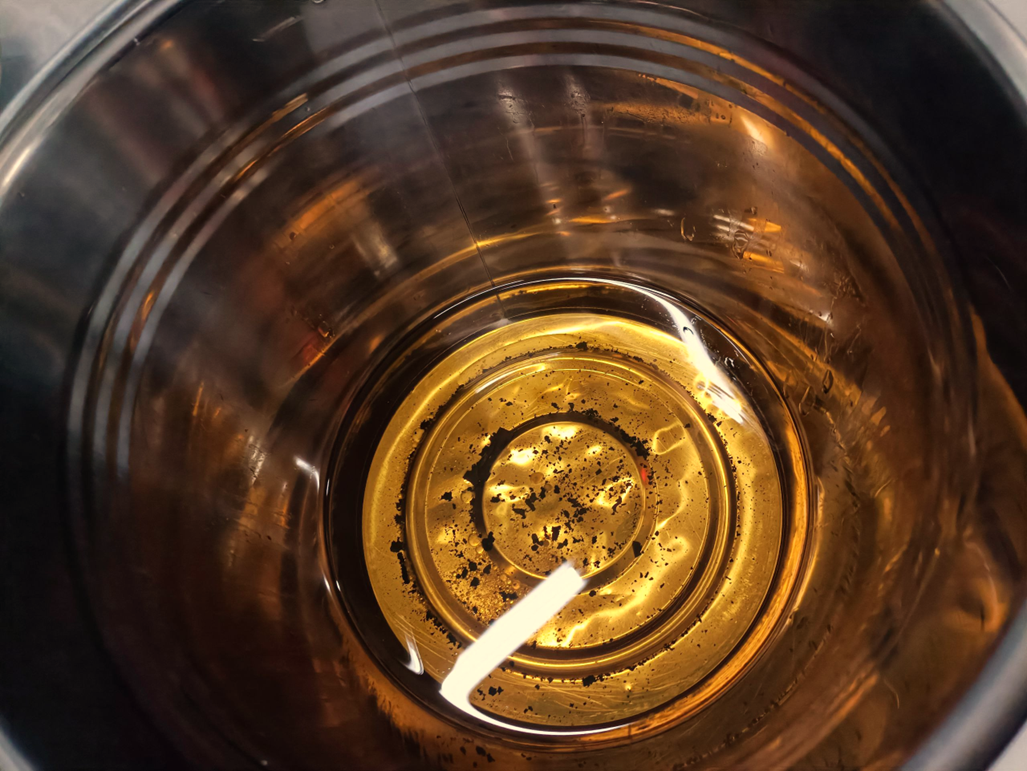
\includegraphics[scale=0.2]{pic/淬火油}}
	\caption{淬火用的液体}
	\label{fig:淬火用液体}
\end{figure}

\subsection{TC4钛合金的热处理方案设计}
\subsection{TC4合金的热处理工艺性能}
在小\ref{sec:1.1}提到过,钛合金可以通过各种各样的相变过程来得到不同的组织结构,所以可根据其固态相变的特点来设计适宜的热处理工艺参数,以获得具有高强度的显微组织,由此实现\ti 合金力学性能和工艺性能的改善。\ti 合金热处理的一些特性如下:
\begin{enumerate}
	%	\item 钛合金的热处理主要用于$\alpha+\beta$型钛合金。因为对于纯α型钛合金而言,马氏体相变不会使钛合金的性能发生显著变化。只能依赖淬火形成的亚稳相(包括马氏体相)的时效分解来进行。
	%	\item 热处理应该避免形成ω相。形成ω相会使钛合金变脆,正确选择时效工艺(例如,采用较高的时效温度)即可使相分解。
	\item $\alpha+\beta$钛合金的淬透性差,淬火热应力大,淬火时零件易翘曲。由于导热性差,钛合金变形时易引起局部温升过高,使局部温度有可能超过$\beta$转变点而形成魏氏组织。
	\item 化学性质活泼。热处理时,钛合金易与氧和水蒸气反应,在工件表面形成具有一定深度的富氧层或氧化皮,使合金的性能降低。同时钛合金热处理时容易吸氢,引起氢脆。
	\item $\beta$转变点差异大。即使是同一成分,但由于冶炼炉次的不同,其$\beta$转变温度有时差别很大。
\end{enumerate}
\subsection{TC4合金热处理工艺设计}
常见的\ti 钛合金热处理工艺有:退火、淬火(往往加上时效处理)、形变热处理等,不同的热处理方式得到的组织性能各异。现阶段\ti 合金的基本热处理工艺主要有:
\begin{enumerate}
	\item 固溶处理:实施固溶处理工艺,是为了得到等轴稳定的$\alpha $相、马氏体弥散的$ \alpha ^{\prime} $相、亚稳定状态的$\beta $相,等轴的$\alpha $相能够让合金的力学性能得到综合性的提升,马氏体弥散的$ \alpha ^{\prime} $相能够让合金,在强度、硬度上得到提高,塑性、韧性被降低\cite{gurong2002}。
	\item 时效处理:次生的$\alpha $相体积分数在TC4钛合金中,会对屈服强度产生很大的影响。在条件相等的情况之下,时效温度越低组织越小,时效温度高低组织越大。研究人员主要是通过控制参数,来影响对次生$\alpha $相的含量,从而实现TC4钛合金强度和塑性的匹配。
	\item 深冷处理:深冷处理是20世纪60年代以来兴起的一种新型冷处理工艺。通过对材料进行-130°C以下的低温处理,可以对金属内部的组织进行改善,并且能够让在热处理之后残留的奥氏体被清除掉。实验研究发现,原始的$\beta $相会在深冷处理的过程当中,逐渐的向$\alpha^{\prime} $相去转变,残余应力在组织中会变少,与此同时网篮状组织的增加,会让TC4钛合金的韧性、强度、塑性,在组织上的性能得到提高。
	\item 氮化处理:常在冷轧后进行氮化处理,TC4在低温氮化过程中会发生重结晶,可以避免晶粒粗化,提高表面强度\cite{guotanliuMicrostructureEvolutionTi2022}。
\end{enumerate}
不同的热处理工艺互相组合可以对合金产生更好的强化效果,现阶段工业上常采用\cite{zhoukaixiangJiyushenlengchulidenanjiagongcailiaoqiexiaotexingyanjiu2022}:淬火+时效;固溶+时效;双重固溶+时效;固溶+双重时效;时效+冷轧+低温氮化等,其中固溶+时效处理是应用最为广泛的一种热处理工艺组合。

对于$\alpha+\beta$型的\ti 钛合金的固溶时效热处理工艺而言,其主要影响参数为固溶、时效的温度和时间\cite{mirror1,ranxingGurongwenduduiTi6Al4VELItaihejinxianweizuzhijixingnengdeyingxiang2021}。


冉兴等人表明\cite{ranxingGurongwenduduiTi6Al4VELItaihejinxianweizuzhijixingnengdeyingxiang2021}在固溶温度为952℃附近时,TC4合金具有较高的强度,但随着温度的升高其脆性增加;鲁媛媛,马保飞等人研究发现在时效温度为450℃、500℃和550℃时初生α相的含量随温度升高逐渐增加;而在时效温度为600℃和650℃条件下初生$\alpha$相含量因高温溶解而明显减少, $\beta$相尺寸相应增大。当时效温度为550℃时, 所得钛合金的显微组织最佳\cite{luyuanyuanShixiaochuliduiTC4taihejinweiguanzuzhihelixuexingnengdeyingxiang2019}。刘婉颖、林元华等人通过实验发现:在960 ℃/1 h + WQ进行固溶处理和500 ℃/4 h + AC下进行时效处理得到的\ti 具有最佳的力学性能\cite{LiuWanYingBuTongReChuLiGongYiDuiTi6Al4VTaiHeJinWeiGuanJieGouHeLiXueXingNengYingXiangYingWen2017};陈冠宇通过实验表明,在850℃进行退火处理时,在600℃进行时效处理可以使合金得到更好的耐腐蚀性能\cite{1200};李宸宇证明\ti 合金在900℃空冷固溶两小时在530℃时效四小时后具有更好的强硬度,而且固溶后冷速越快,合金的强硬度越高、塑韧性越差\cite{900}。%第46页


根据以上研究者的观点,初步预测确定了固溶处理的最佳工艺制度为$ \beta $相变点以下30℃左右(这里取整数$ 977.325-30=947.325\approx950^{\circ} \mathrm{C} $)处理一个小时、时效温度在450℃左右处理一个小时。经过研读,发现现阶段鲜对固溶冷却速度影响作用研究。于是本设计综合考量各个因素,设置了如下三个变量:固溶温度、固溶冷却方式(冷速)、时效温度来研究其对合金组织性能的影响。

根据控制变量法,本设计初步设计了如\ref{sec:first}所示的18组热处理实验:
\begin{table}[htbp]
	\centering
	\caption{以控制变量法为原则的热处理制度设计}
	\label{sec:first}
	\begin{tabular}{cccccc}
		\toprule
		固溶温度/℃ &处理时间/h & 冷却方法 & 时效温度/℃  &处理时间/h & 冷却方法 \\
		\midrule
		910 & 1 & $\mathrm{WQ}$ & 510 & 4 & $\mathrm{AC}$\\
		910 & 1 & $\mathrm{FC}$  & 510 & 4 & $\mathrm{AC}$ \\
		910 & 1 & $\mathrm{WQ}$ & 550 & 4 & $\mathrm{AC}$ \\
		910 & 1 & $\mathrm{FC}$  & 550 & 4 & $\mathrm{AC}$ \\
		910 & 1 & $\mathrm{WQ}$ & 590 & 4 & $\mathrm{AC}$ \\
		910 & 1 & $\mathrm{FC}$  & 590 & 4 & $\mathrm{AC}$ \\
		\midrule
		950 & 1 & $\mathrm{WQ}$ & 510 & 4 & $\mathrm{AC}$ \\
		950 & 1 & $\mathrm{FC}$ & 510 & 4 & $\mathrm{AC}$ \\
		950 & 1 & $\mathrm{WQ}$ & 550 & 4 & $\mathrm{AC}$ \\
		950 & 1 & $\mathrm{FC}$ & 550 & 4 & $\mathrm{AC}$ \\
		950 & 1 & $\mathrm{WQ}$ & 590 & 4 & $\mathrm{AC}$ \\
		950 & 1 & $\mathrm{FC}$ & 590 & 4 & $\mathrm{AC}$ \\
		\midrule
		990 & 1 & $\mathrm{WQ}$ & 510 & 4 & $\mathrm{AC}$ \\
		990 & 1 & $\mathrm{FC}$ & 510 & 4 & $\mathrm{AC}$ \\
		990 & 1 & $\mathrm{WQ}$ & 550 & 4 & $\mathrm{AC}$ \\
		990 & 1 & $\mathrm{FC}$ & 550 & 4 & $\mathrm{AC}$ \\
		990 & 1 & $\mathrm{WQ}$ & 590 & 4 & $\mathrm{AC}$ \\
		990 & 1 & $\mathrm{FC}$ & 590 & 4 & $\mathrm{AC}$ \\
		\bottomrule
	\end{tabular}
\end{table}

控制变量法是科学实验中最常使用的方法,在面对低因素、低水平的实验时可以设计出很清晰直观的实验。但其也存在巨大的缺点,尤其是多个因素交互作用的影响,面对多因素(变量)、多水平的实验时,就需要设计很多次的实验,显得极为繁琐。比如一个含有三个变量,每个变量有三个水平的实验就需要$ 3\times 3 \times 3=27$次实验,为了直观性而牺牲大量的成本、同时包含了太多无关的对照组,这样的实验设计在很大程度上是不符合可持续发展理念的,是在浪费资源。但好在有另外一种方法可以解决问题——正交试验设计法(Orthogonal experimental design)。

正交实验设计是研究多因素多水平的又一种设计方法,可以用更少的试验次数来研究多个变量之间的关系。它是根据正交性从全面试验中挑选出部分有代表性的点进行试验,这些有代表性的点具备了“均匀分散,齐整可比”的特点\cite{wangxueshen}。当实验次数太多时,根据正交实验设计,实验者可以选择一部分有代表性水平组合进行试验。 例如前面说的三因素三水平的实验,若按$ L9(3^4) $正交表安排实验,只需作9次,按$ L15(3^7) $正交表进行15次实验,就可以大大减少试验次数,提高实验效率、材料利用率。


在没有通过正交实验设计优化之前,笔者的实验是如\ref{sec:first}所示,需要做$3\times2\times3  =18$次实验。但为了给子孙后代留下天蓝、地绿、水清的美丽家园,本实验高举可持续发展理念伟大旗帜,结合了正交实验方法$\color{black} L9.3.4 $对实验进行了优化,最终的热处理制度如下表所示:%\footnote{其中WQ表示水冷、FC表示炉冷、AC表示空冷。}
\begin{table}[htbp]
	\centering
	\caption{经过正交实验法改进后的最终热处理制度}
	\label{sec:myHT}
	\resizebox{\linewidth}{!}{
		\begin{tabular}{ccccccc}
			\toprule
			实验编号&固溶温度/℃ &处理时间/h & 冷却方法 & 时效温度/℃  &处理时间/h & 冷却方法 \\
			\midrule
			1 & 910 & 1 & 水冷 & 510 & 1 & AC \\
			2 & 910 & 1 & 油冷 & 590 & 1 & AC \\
			3 & 910 & 1 & 水冷 & 550 & 1 & AC \\
			4 & 950 & 1 & 水冷 & 590 & 1& AC \\
			5 & 950 & 1 & 水冷 & 550 & 1& AC \\
			6 & 950 & 1 & 油冷 & 510 & 1 & AC \\
			7 & 990 & 1 & 水冷 & 550 & 1 & AC \\
			8 & 990 & 1 & 油冷 & 510 & 1 & AC \\
			9 & 990 & 1 & 水冷 & 590 & 1 & AC \\
			%	910 & 1 & $\mathrm{WQ}$ & 510 & 4 & $\mathrm{AC}$\\
			%	910 & 1 & $\mathrm{FC}$  & 510 & 4 & $\mathrm{AC}$ \\
			%	910 & 1 & $\mathrm{WQ}$ & 550 & 4 & $\mathrm{AC}$ \\
			%	910 & 1 & $\mathrm{FC}$  & 550 & 4 & $\mathrm{AC}$ \\
			%	910 & 1 & $\mathrm{WQ}$ & 590 & 4 & $\mathrm{AC}$ \\
			%	910 & 1 & $\mathrm{FC}$  & 590 & 4 & $\mathrm{AC}$ \\
			%	\midrule
			%	950 & 1 & $\mathrm{WQ}$ & 510 & 4 & $\mathrm{AC}$ \\
			%	950 & 1 & $\mathrm{FC}$ & 510 & 4 & $\mathrm{AC}$ \\
			%	950 & 1 & $\mathrm{WQ}$ & 550 & 4 & $\mathrm{AC}$ \\
			%	950 & 1 & $\mathrm{FC}$ & 550 & 4 & $\mathrm{AC}$ \\
			%	950 & 1 & $\mathrm{WQ}$ & 590 & 4 & $\mathrm{AC}$ \\
			%	950 & 1 & $\mathrm{FC}$ & 590 & 4 & $\mathrm{AC}$ \\
			%	\midrule
			%	990 & 1 & $\mathrm{WQ}$ & 510 & 4 & $\mathrm{AC}$ \\
			%	990 & 1 & $\mathrm{FC}$ & 510 & 4 & $\mathrm{AC}$ \\
			%	990 & 1 & $\mathrm{WQ}$ & 550 & 4 & $\mathrm{AC}$ \\
			%	990 & 1 & $\mathrm{FC}$ & 550 & 4 & $\mathrm{AC}$ \\
			%	990 & 1 & $\mathrm{WQ}$ & 590 & 4 & $\mathrm{AC}$ \\
			%	990 & 1 & $\mathrm{FC}$ & 590 & 4 & $\mathrm{AC}$ \\
			\bottomrule
		\end{tabular}
	}
\end{table}

%\subsection{正交实验分析方法}
%经过正交实验方法设计的实验虽然节省了试验次数,但是不能兼顾直观性,因而需要专门的分析工具才能分析出来,不同变量之间的相关性,故本实验采用spssau提供的数据分析工具来对三因素影响结果进行分析。

%{\Huge \color{red} \textbf {待补充}}

\subsection{固溶时效处理实验过程}
\begin{enumerate}
	\item 设备与试样准备:把样品用去离子水等清洗干净,确保表面干净无杂质,无水分。准备陶瓷样品架,以便样品可以均匀加热。准备好后,将热处理炉预热至900℃左右,并保持稳定。
	\item 样品装入:将切好的样品用放置在样品架上,不要使样品直接接触炉子底部或顶部,以免影响加热效果。并确保样品间距均匀,并记录好摆放顺序。
	\item 加热过程控制:将样品架或钛合金网放入炉中,启动加热程序。根据实验要求,控制加热速率、温度和保温时间等参数(这里分三批次\textbf{910-950-990},每批次六个试样进行处理)。
	\item 保温时间控制:加热到设计的温度后后,让试样保温一段时间,使其完全进入固溶状态。保持加热系统稳定,避免温度波动。
	\item 停止加热:当固溶处理时间{\footnote{由于试样过小,为了节约资源,实际加热只进行了10分钟}}到达后,停止加热并关闭加热系统,取出处理好的试样。
	\item 水淬或油淬:将处理后的样品快速分别浸入水中、淬火油中进行淬火(每批次四个水淬,两个油淬)。
	\item 后处理:取出样品进行干燥、清洗、归类,并记录初步记录数据。
\end{enumerate}
经过固溶时效处理后的试样如图所示:

\begin{figure}[h!]
	\centering
	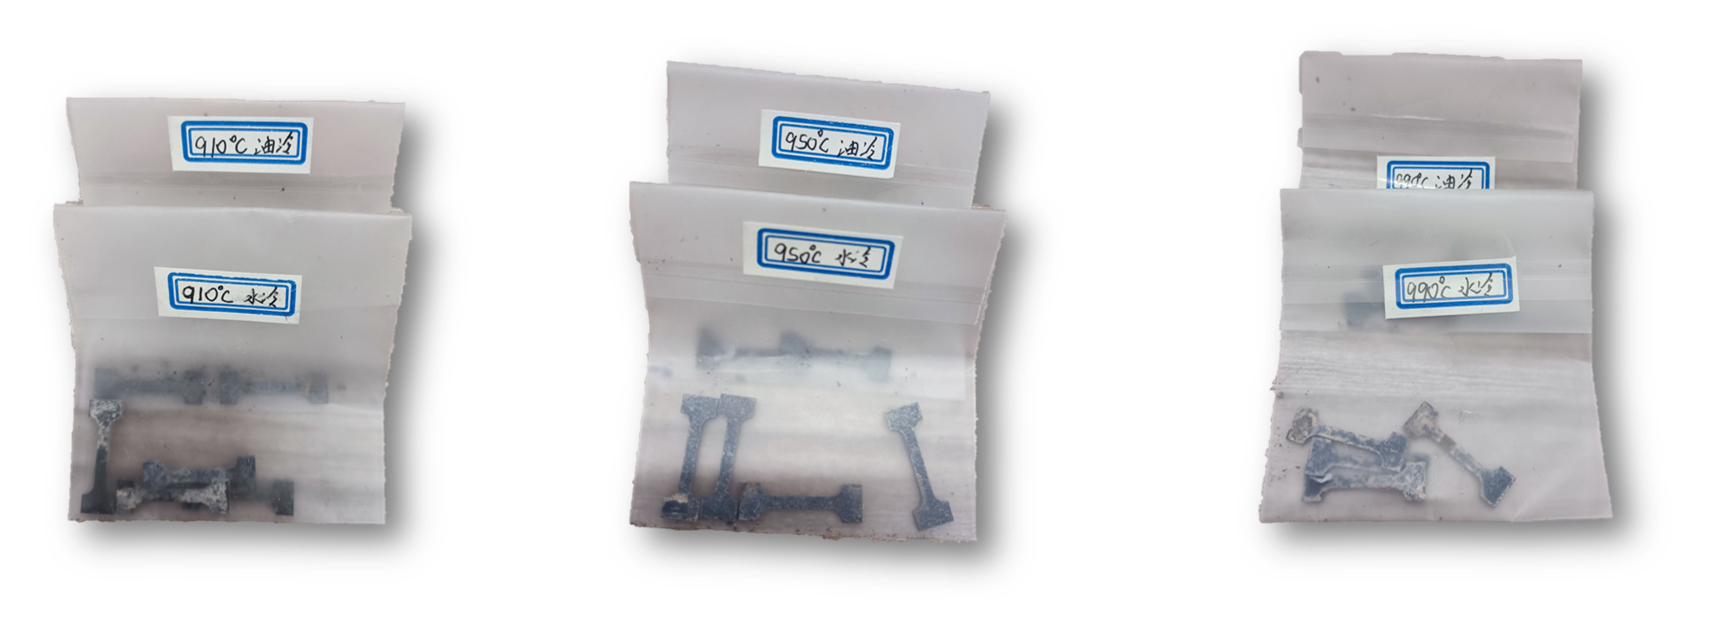
\includegraphics[width=0.8\linewidth]{pic/固溶处理后的试样}
	\caption{固溶处理后的试样}
	\label{fig: aftergurong}
\end{figure}

时效处理过程温度稍低,为\textbf{510-550-590}三个温度,冷却方式为空冷,具体步骤与固溶处理相同,在此不做赘述。

处理后,使用砂纸将表面氧化层打磨干净,根据试样所处的不同工艺路线,将各个试样分组归类。

%\section{小结}
%在本节中,介绍了式样的参数与加工过程与热处理工艺的设计

\section{室温力学拉伸试验}
力学性能是表征材料性能的重要参数,本次试验\footnote{实验(Experiment)是通过实际操作来探究某一自然或社会规律,主要强调与理论研究的方法对立;而试验(test)采用测试的手段来获取或验证某一结果的行为。此处当为“试验”。}采用常规的拉伸试验来测量式样的力学性能。力学拉伸试验是一种常用的材料力学性能测试方法,用于评估材料的抗拉性能、塑性性能和断裂性能等。其主要特点是通过拉伸试验机对试样进行一定的力量加载和拉伸,测量试样在不同载荷下的应变和应力,以此计算出力学特性参数,如屈服强度、抗拉强度、延伸率等。该测试方法简单、直观,结果可靠,并可以广泛应用于各种材料试样的力学性能评估。本试验根据拉伸试验主要根据测量结果来评估材料的如下四个力学性能指标:
\begin{enumerate}
	\item 屈服强度:表示材料在开始发生可见塑性变形前的最大应力值。
	\item 抗拉强度:表示材料在断裂前所能承受的最大应力值。
	\item 断裂应变:表示材料在断裂发生前所受的最大应变值。
	\item 延伸率:表示材料在断裂前可以发生的塑性变形程度,是反映材料延展性能的指标\footnote{由于试样较小,测量误差大,本设计主要考虑沿拉伸方向的延伸率来分析正应力与正应变,断裂截面较小,界面面积与切应力难以测量,为了保证试验整体的准确性,不对其进行探讨。}。
\end{enumerate}

本设计采用拉伸试验机对经固溶时效热处理工艺的试样进行常温微拉伸性能测试。由于试样较小,冲击韧性较差,容易被拉断,为了尽可能准确地观察其力学特性,采用了较慢的$ 0.5mm/min $的拉伸速率来拉伸,每组试样进行两次测定,取其平均值作为最终结果。所用的设备为\text{\color{black}CMT5105}微机控制电子万能试验机(Electromechaniacl Universal Testing Machine),外观如\ref{fig:mymechyest}所示,设备规格如\ref{sec: mymechyest}所示:
\begin{table}[htbp]
	\centering
	\caption{\text{\color{black}CMT5105}微机控制电子万能试验机的规格}
	\label{sec: mymechyest}
	\begin{tabular}{cc}
		\toprule
		参数&值\\
		\midrule
		型号&CMT5105\\
		编号&17020836\\
		电压&三相 380VAC\\
		功率&1.3KW\\
		最大力&100kN\\
		准确度等级&0.5级\\
		制造日期&2022年8月\\
		制造商& $\text{美斯特工业系统}^\text{\textregistered} $(中国)有限公司\\
		\bottomrule
	\end{tabular}
\end{table}

\begin{figure}[h!]
	\centering
	\subfigure[力学试验机]{
		\label{fig:mymechyest}
		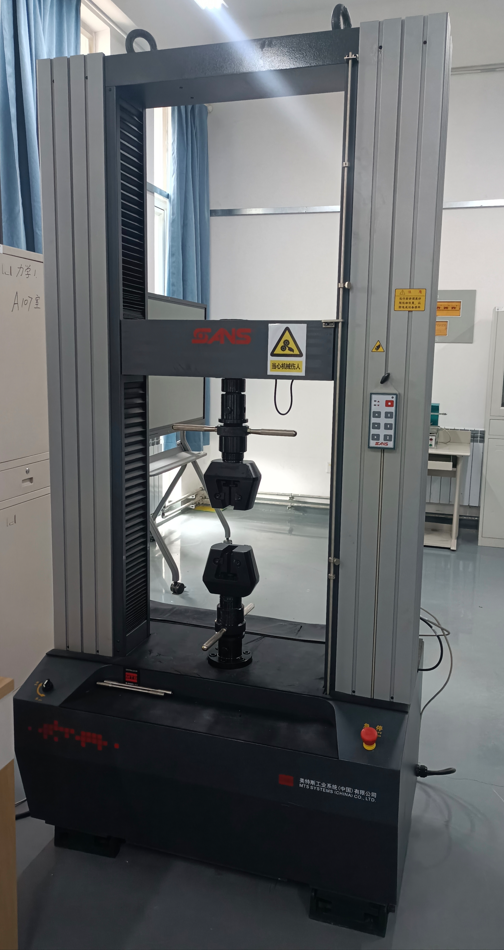
\includegraphics[scale=0.4]{pic/力学试验机}}
	\hspace{0.5in} % 两图片之间的距离
	\subfigure[试样安装]{
		\label{fig:mytest}
		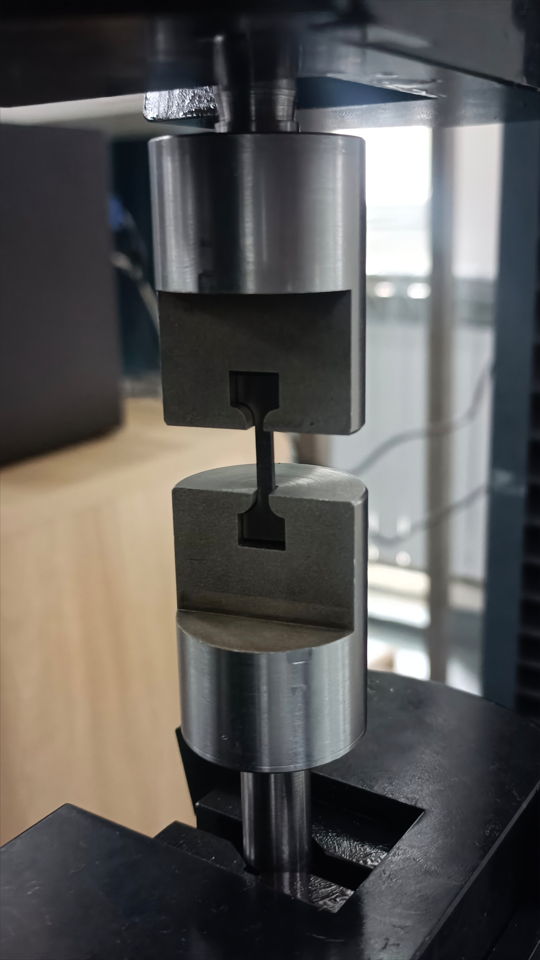
\includegraphics[scale=0.4]{pic/拉伸试验}}
	\caption{拉伸试验}
	\label{fig:拉伸试验}
\end{figure}

\subsection{试验流程}
试验前,先准备好试样,在试样上刻上标记,以确定试样的方向。然后如图\ref{fig:拉伸试验}在拉伸试验机上安装试样,并在拉伸试验机上设置截面尺寸、最大加载力、加载速率等参数。

一次拉伸试验包括两个阶段:弹性阶段和塑性阶段。弹性阶段是指当外力作用在试样上时,试样的形变是可逆的,即当外力消失时,试样会完全恢复其原始尺寸。随着外力的增加,试样进入塑性阶段,此时试样发生不可逆的塑性变形,当外力达到试样的最大强度时,试样会断裂。

试验时,对试样采用一次性拉断的方式来进行测试,并通过传感器,利用计算机来记录其载荷-位移曲线,导出数据进行分析。

最后通过测量式样拉断后的长度,计算得到延伸率。

\subsection{拉伸试验结果分析}
根据对万能力学试验机上测试得到的数据进行整理,得到了抗拉强度\footnote{根据《金属材料室温拉伸试验方法》GBT228-2002,抗拉强度符号已经由$ R_m $代替旧国标中的$ \sigma_b $,故在此使用最新标准$ R_m $来表示抗拉强度。}、延伸率,如\ref{sec:mystrength}所示。又通过去除力学试验数据中从断裂瞬间到试验结束之间的无用数值、整合每组两个试验结果(取平均值),计算得到了试样断裂区域截面($ 1.3mm\times2.5mm=3.25mm^2 $)的应力与应变曲线(拉伸变形量与拉伸区域长度的比值),最后把包括未处理的对照组在内的十组数据的应力应变曲线进行汇总,得到了如\ref{fig:试样应力应变曲线汇总}\footnote{图形中标签未标明的,所有组共同具有工艺参数为:固溶处理时间:10分钟;时效处理时间:60分钟}所示的可视化图形:
\begin{table}[htbp]
	\centering
	\caption{\ti 合金的力学性能试验结果}
	\label{sec:mystrength}
	\begin{tabular}{cccc}
		\toprule
		试验编号& 代号&$ R_m $(Mpa)&延伸率 \\
		\midrule
		0 & 甲 & 1008.69 & 6.83$\%$ \\
		1 & 乙 & 1188.36 & 3.73$\%$ \\
		2 & 丙 & 1077.33 & 4.24$\%$ \\
		3 & 丁 & 1094.87 & 3.49$\%$ \\
		4 & 戊 & 1099.33 & 2.60$\%$ \\
		5 & 己 & 1113.90 & 2.57$\%$ \\
		6 & 庚 & 1077.28 & 2.88$\%$ \\
		7 & 辛 & 790.10 & 1.94$\%$ \\
		8 & 壬 & 799.54 & 2.05$\%$ \\
		9 & 癸 & 873.38 & 2.19$\%$ \\
		\bottomrule
	\end{tabular}
\end{table}
\begin{figure}[h!]
	\centering
	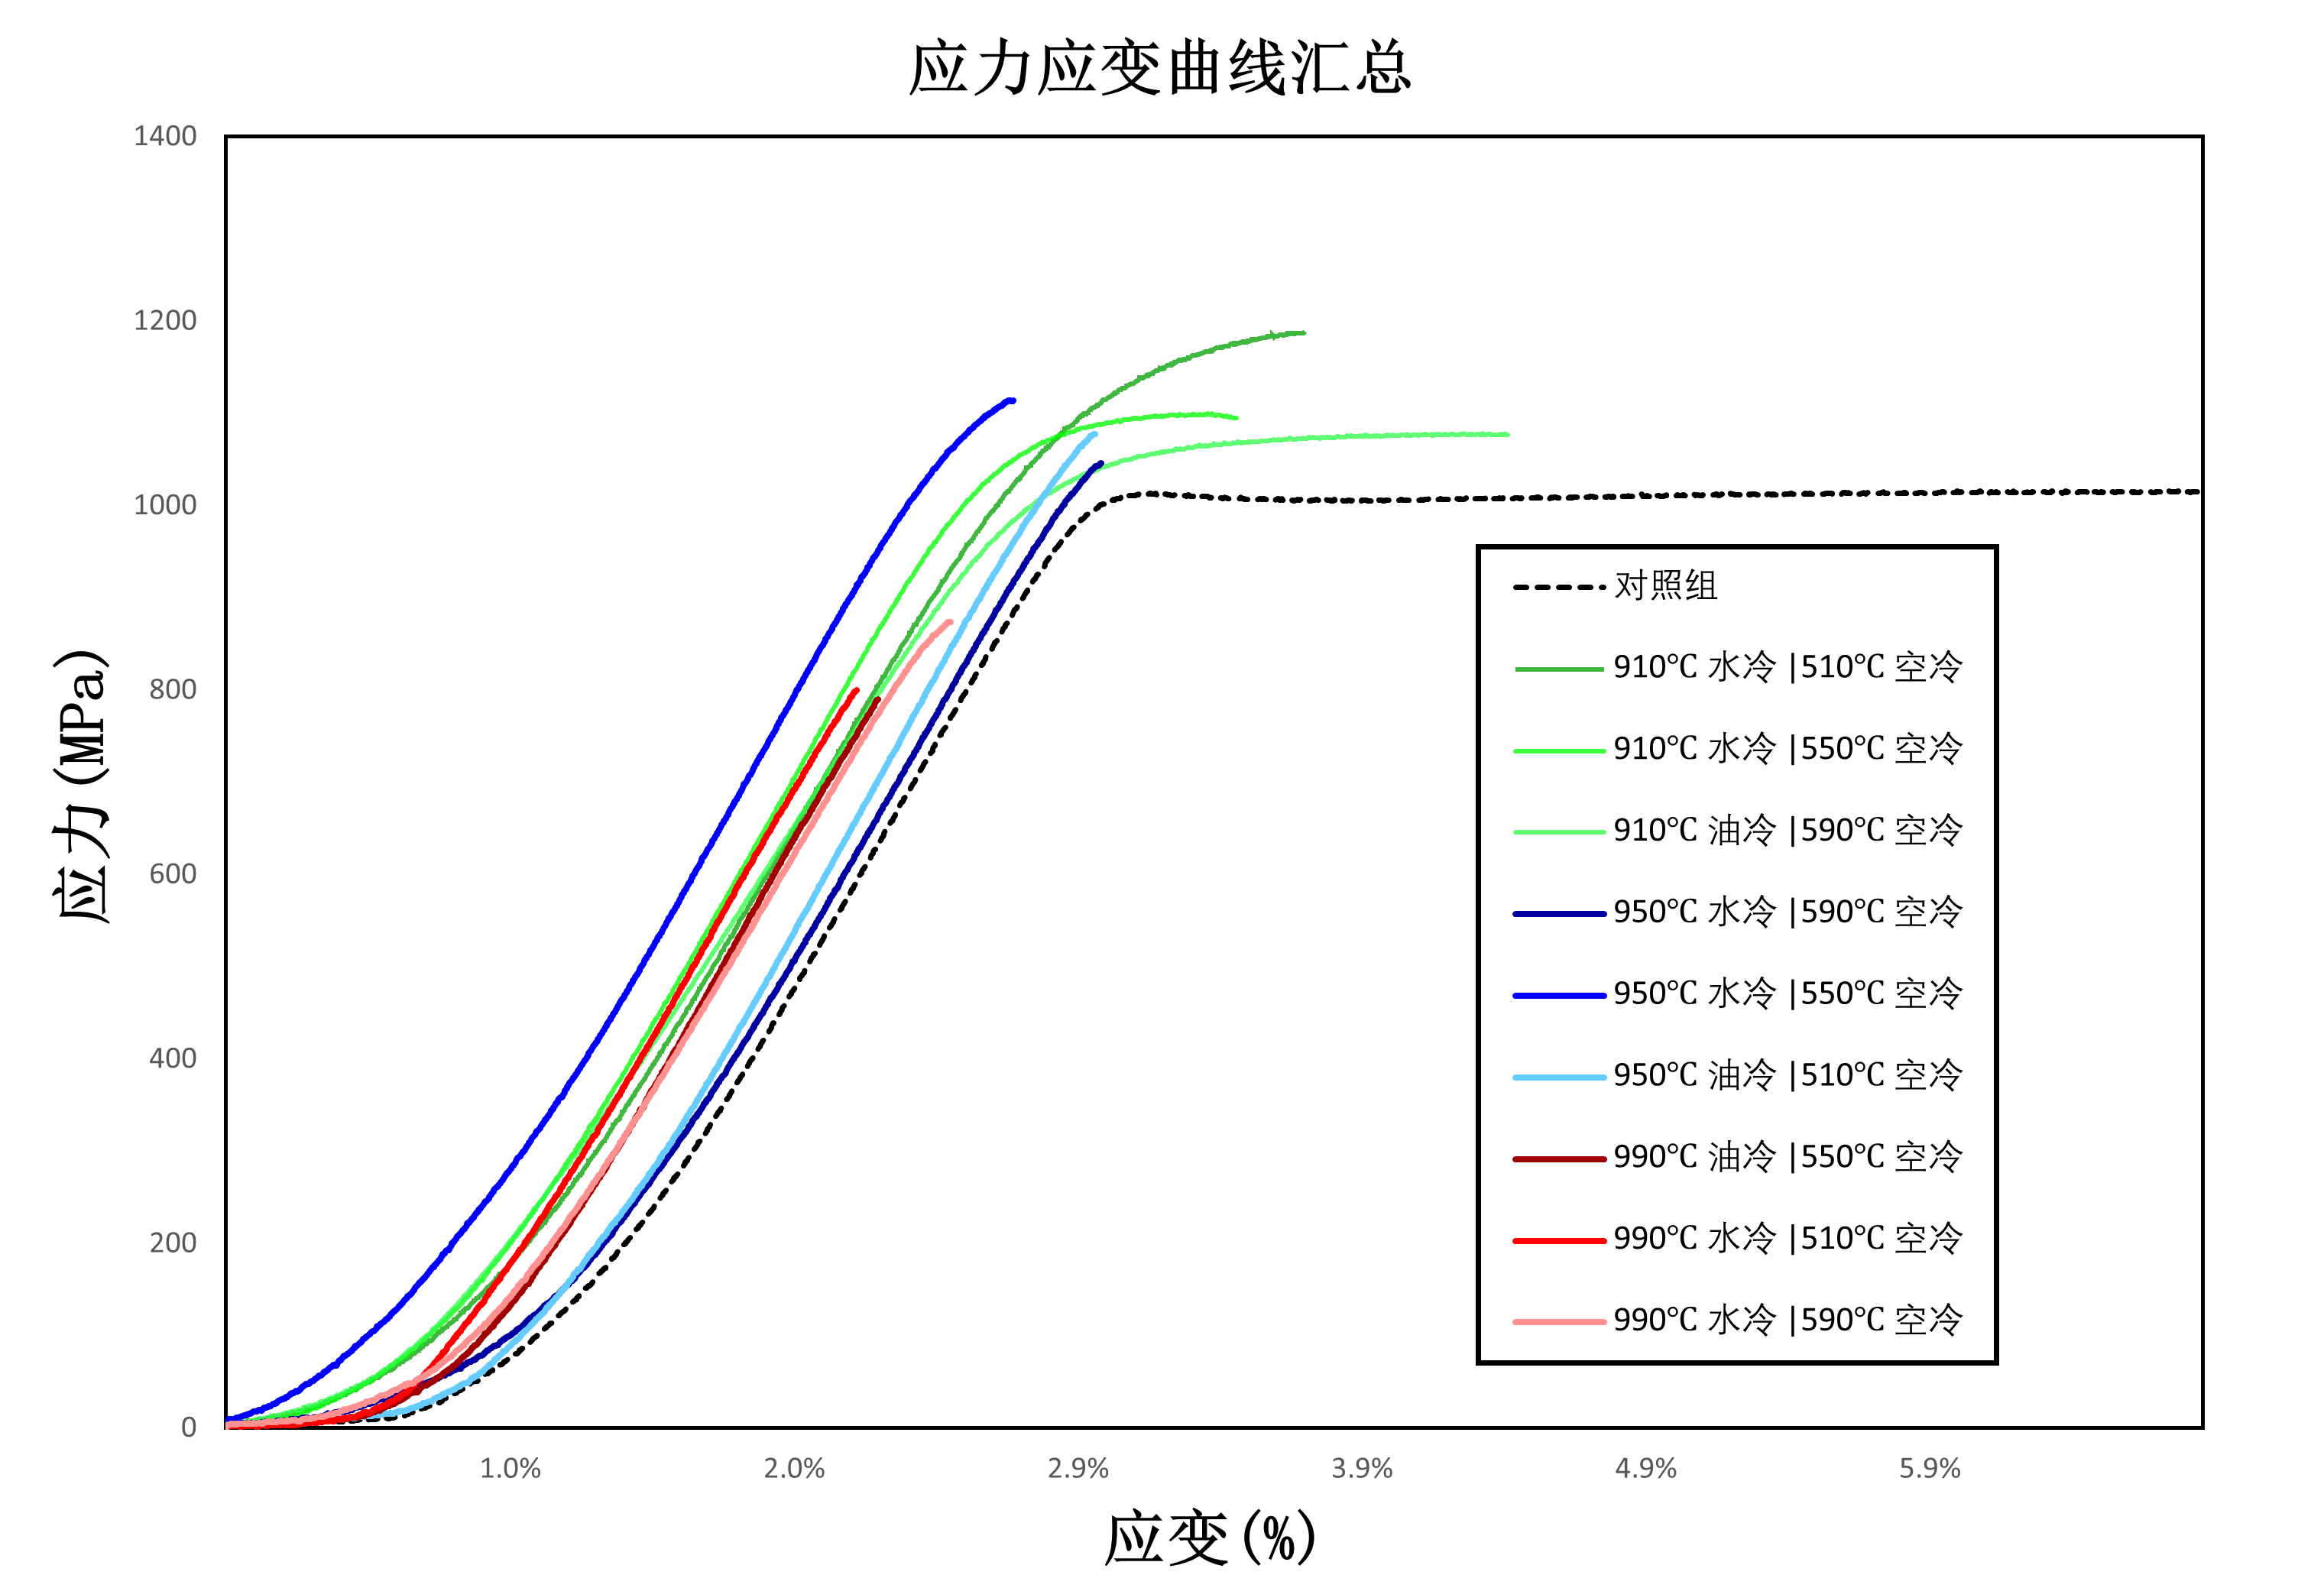
\includegraphics[width=0.99\linewidth]{pic/试样应力应变曲线汇总.png}
	\caption{试样应力应变曲线汇总}
	\label{fig:试样应力应变曲线汇总}
\end{figure}
\section{组织观察与相结构分析}
现阶段常用于观察组织和分析相结构的检测方法主要包括:光学显微镜 (OM)、扫描式电子显微镜 (SEM)、X射线衍射分析 (XRD)以及透射式电子显微镜 (TEM)等。

将固溶与时效后的试件进行线切割截取显微组织分析试样,截取后的试样进行 150\#、400\#、1000\#、1500\#、2000\#、2500\#金相砂纸磨制,对磨制后的试样采用 0.05umSiO2抛光液在抛光机上进行抛光,去除试样表面的划痕或杂质颗粒,经抛光后的试样采用$ HF:HNO3:H2O=2:4:94 $的Kroll试剂进行腐蚀。腐蚀后的试样分别采用光 学显微镜(OM)、扫描电子显微镜(SEM)对其微观形貌进行观察。
